\documentclass[twoside]{book}

% Packages required by doxygen
\usepackage{fixltx2e}
\usepackage{calc}
\usepackage{doxygen}
\usepackage{graphicx}
\usepackage[utf8]{inputenc}
\usepackage{makeidx}
\usepackage{multicol}
\usepackage{multirow}
\PassOptionsToPackage{warn}{textcomp}
\usepackage{textcomp}
\usepackage[nointegrals]{wasysym}
\usepackage[table]{xcolor}

% NLS support packages
\usepackage[spanish]{babel}
% Font selection
\usepackage[T1]{fontenc}
\usepackage{mathptmx}
\usepackage[scaled=.90]{helvet}
\usepackage{courier}
\usepackage{amssymb}
\usepackage{sectsty}
\renewcommand{\familydefault}{\sfdefault}
\allsectionsfont{%
  \fontseries{bc}\selectfont%
  \color{darkgray}%
}
\renewcommand{\DoxyLabelFont}{%
  \fontseries{bc}\selectfont%
  \color{darkgray}%
}
\newcommand{\+}{\discretionary{\mbox{\scriptsize$\hookleftarrow$}}{}{}}

% Page & text layout
\usepackage{geometry}
\geometry{%
  a4paper,%
  top=2.5cm,%
  bottom=2.5cm,%
  left=2.5cm,%
  right=2.5cm%
}
\tolerance=750
\hfuzz=15pt
\hbadness=750
\setlength{\emergencystretch}{15pt}
\setlength{\parindent}{0cm}
\setlength{\parskip}{0.2cm}
\makeatletter
\renewcommand{\paragraph}{%
  \@startsection{paragraph}{4}{0ex}{-1.0ex}{1.0ex}{%
    \normalfont\normalsize\bfseries\SS@parafont%
  }%
}
\renewcommand{\subparagraph}{%
  \@startsection{subparagraph}{5}{0ex}{-1.0ex}{1.0ex}{%
    \normalfont\normalsize\bfseries\SS@subparafont%
  }%
}
\makeatother

% Headers & footers
\usepackage{fancyhdr}
\pagestyle{fancyplain}
\fancyhead[LE]{\fancyplain{}{\bfseries\thepage}}
\fancyhead[CE]{\fancyplain{}{}}
\fancyhead[RE]{\fancyplain{}{\bfseries\leftmark}}
\fancyhead[LO]{\fancyplain{}{\bfseries\rightmark}}
\fancyhead[CO]{\fancyplain{}{}}
\fancyhead[RO]{\fancyplain{}{\bfseries\thepage}}
\fancyfoot[LE]{\fancyplain{}{}}
\fancyfoot[CE]{\fancyplain{}{}}
\fancyfoot[RE]{\fancyplain{}{\bfseries\scriptsize Generado el Viernes, 3 de Marzo de 2017 13\+:12\+:32 para Práctica 1 -\/ S\+O\+P\+E\+R por Doxygen }}
\fancyfoot[LO]{\fancyplain{}{\bfseries\scriptsize Generado el Viernes, 3 de Marzo de 2017 13\+:12\+:32 para Práctica 1 -\/ S\+O\+P\+E\+R por Doxygen }}
\fancyfoot[CO]{\fancyplain{}{}}
\fancyfoot[RO]{\fancyplain{}{}}
\renewcommand{\footrulewidth}{0.4pt}
\renewcommand{\chaptermark}[1]{%
  \markboth{#1}{}%
}
\renewcommand{\sectionmark}[1]{%
  \markright{\thesection\ #1}%
}

% Indices & bibliography
\usepackage{natbib}
\usepackage[titles]{tocloft}
\setcounter{tocdepth}{3}
\setcounter{secnumdepth}{5}
\makeindex

% Hyperlinks (required, but should be loaded last)
\usepackage{ifpdf}
\ifpdf
  \usepackage[pdftex,pagebackref=true]{hyperref}
\else
  \usepackage[ps2pdf,pagebackref=true]{hyperref}
\fi
\hypersetup{%
  colorlinks=true,%
  linkcolor=blue,%
  citecolor=blue,%
  unicode%
}

% Custom commands
\newcommand{\clearemptydoublepage}{%
  \newpage{\pagestyle{empty}\cleardoublepage}%
}


%===== C O N T E N T S =====

\begin{document}

% Titlepage & ToC
\hypersetup{pageanchor=false,
             bookmarks=true,
             bookmarksnumbered=true,
             pdfencoding=unicode
            }
\pagenumbering{roman}
\begin{titlepage}
\vspace*{7cm}
\begin{center}%
{\Large Práctica 1 -\/ S\+O\+P\+E\+R }\\
\vspace*{1cm}
{\large Generado por Doxygen 1.8.7}\\
\vspace*{0.5cm}
{\small Viernes, 3 de Marzo de 2017 13:12:32}\\
\end{center}
\end{titlepage}
\clearemptydoublepage
\tableofcontents
\clearemptydoublepage
\pagenumbering{arabic}
\hypersetup{pageanchor=true}

%--- Begin generated contents ---
\chapter{Indice de archivos}
\section{Lista de archivos}
Lista de todos los archivos documentados y con descripciones breves\+:\begin{DoxyCompactList}
\item\contentsline{section}{\hyperlink{ejercicio10_8c}{ejercicio10.\+c} \\*Fuente del ejercicio 10 }{\pageref{ejercicio10_8c}}{}
\item\contentsline{section}{\hyperlink{ejercicio10b_8c}{ejercicio10b.\+c} \\*Fuente del ejercicio 10, versión2 }{\pageref{ejercicio10b_8c}}{}
\item\contentsline{section}{\hyperlink{ejercicio3a_8c}{ejercicio3a.\+c} \\*Fuente del ejercicio 3a }{\pageref{ejercicio3a_8c}}{}
\item\contentsline{section}{\hyperlink{ejercicio3b_8c}{ejercicio3b.\+c} \\*Fuente del ejercicio 3b }{\pageref{ejercicio3b_8c}}{}
\item\contentsline{section}{\hyperlink{ejercicio4_8c}{ejercicio4.\+c} \\*Fuente del ejercicio 4 Este programa pide al usuario dos matrices y dos factores para multiplicarlas. Multiplica cada una por un factor en dos hilos distintos que además mantienen una comunicación para saber por donde va el otro }{\pageref{ejercicio4_8c}}{}
\item\contentsline{section}{\hyperlink{ejercicio8_8c}{ejercicio8.\+c} \\*Fuente del ejercicio 8 Este programa pide al usuario un número de procesos y un número de vueltas, estos procesos se pasarán una señal tantas vueltas como pida el usuario. Cada vez que uno la recibe, imprime la hora. Finalmente se acaban uno a uno }{\pageref{ejercicio8_8c}}{}
\end{DoxyCompactList}

\chapter{Documentación de archivos}
\hypertarget{ejercicio4a_8c}{\section{Referencia del Archivo ejercicio4a.\+c}
\label{ejercicio4a_8c}\index{ejercicio4a.\+c@{ejercicio4a.\+c}}
}


Fuente del ejercicio 4.  


{\ttfamily \#include $<$stdio.\+h$>$}\\*
{\ttfamily \#include $<$stdlib.\+h$>$}\\*
{\ttfamily \#include $<$unistd.\+h$>$}\\*
{\ttfamily \#include $<$sys/types.\+h$>$}\\*
{\ttfamily \#include $<$sys/wait.\+h$>$}\\*
Dependencia gráfica adjunta para ejercicio4a.\+c\+:
\nopagebreak
\begin{figure}[H]
\begin{center}
\leavevmode
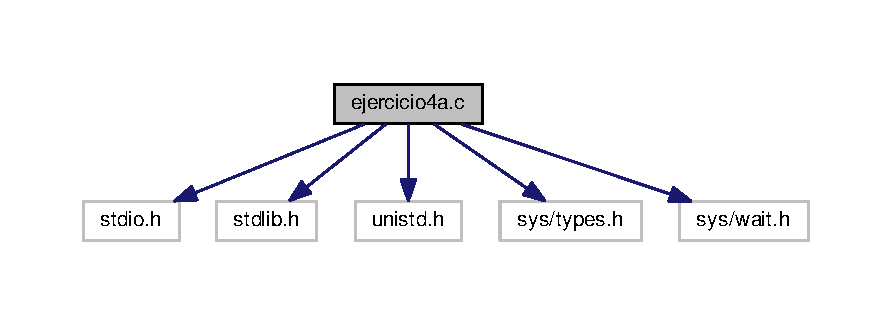
\includegraphics[width=350pt]{ejercicio4a_8c__incl}
\end{center}
\end{figure}
\subsection*{'defines'}
\begin{DoxyCompactItemize}
\item 
\hypertarget{ejercicio4a_8c_acee2369f62e4a096d243dec3cd7d0b00}{\#define {\bfseries N\+U\+M\+\_\+\+P\+R\+O\+C}~3}\label{ejercicio4a_8c_acee2369f62e4a096d243dec3cd7d0b00}

\end{DoxyCompactItemize}
\subsection*{Funciones}
\begin{DoxyCompactItemize}
\item 
\hypertarget{ejercicio4a_8c_a840291bc02cba5474a4cb46a9b9566fe}{int {\bfseries main} (void)}\label{ejercicio4a_8c_a840291bc02cba5474a4cb46a9b9566fe}

\end{DoxyCompactItemize}


\subsection{Descripción detallada}
Fuente del ejercicio 4. 

Este modulo hace una serie de forks e imprime los pid del padre y del hijo de cada uno de estos.

\begin{DoxyAuthor}{Autor}
Pareja 21\+: Juan Riera Gomez (\href{mailto:juan.riera@estudiante.uam.es}{\tt juan.\+riera@estudiante.\+uam.\+es}) y Carlos Ignacio Isasa Martín (\href{mailto:carlos.isasa@estudiante.uam.es}{\tt carlos.\+isasa@estudiante.\+uam.\+es}) 
\end{DoxyAuthor}
\begin{DoxyVersion}{Versión}
1.\+0 
\end{DoxyVersion}
\begin{DoxyDate}{Fecha}
02-\/03-\/2017 
\end{DoxyDate}

\hypertarget{ejercicio4b_8c}{\section{Referencia del Archivo ejercicio4b.\+c}
\label{ejercicio4b_8c}\index{ejercicio4b.\+c@{ejercicio4b.\+c}}
}


Fuente del ejercicio 4, apartado b.  


{\ttfamily \#include $<$stdio.\+h$>$}\\*
{\ttfamily \#include $<$stdlib.\+h$>$}\\*
{\ttfamily \#include $<$unistd.\+h$>$}\\*
{\ttfamily \#include $<$sys/types.\+h$>$}\\*
{\ttfamily \#include $<$sys/wait.\+h$>$}\\*
Dependencia gráfica adjunta para ejercicio4b.\+c\+:
\nopagebreak
\begin{figure}[H]
\begin{center}
\leavevmode
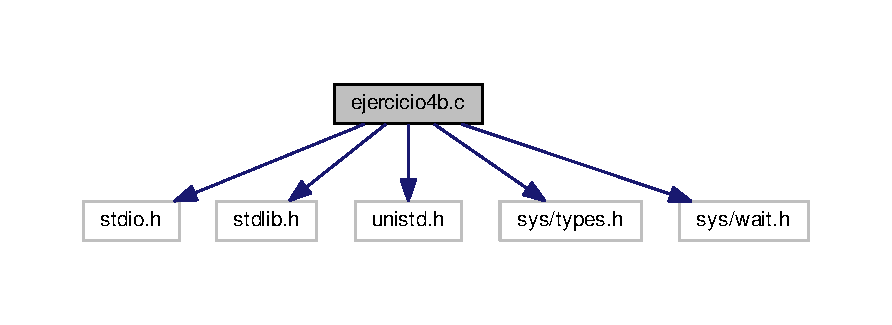
\includegraphics[width=350pt]{ejercicio4b_8c__incl}
\end{center}
\end{figure}
\subsection*{'defines'}
\begin{DoxyCompactItemize}
\item 
\hypertarget{ejercicio4b_8c_acee2369f62e4a096d243dec3cd7d0b00}{\#define {\bfseries N\+U\+M\+\_\+\+P\+R\+O\+C}~3}\label{ejercicio4b_8c_acee2369f62e4a096d243dec3cd7d0b00}

\end{DoxyCompactItemize}
\subsection*{Funciones}
\begin{DoxyCompactItemize}
\item 
\hypertarget{ejercicio4b_8c_a840291bc02cba5474a4cb46a9b9566fe}{int {\bfseries main} (void)}\label{ejercicio4b_8c_a840291bc02cba5474a4cb46a9b9566fe}

\end{DoxyCompactItemize}


\subsection{Descripción detallada}
Fuente del ejercicio 4, apartado b. 

Este modulo hace una serie de forks e imprime los pid del padre y del hijo de cada uno de estos. Además el padre espera a que sus hijos terminen

\begin{DoxyAuthor}{Autor}
Pareja 21\+: Juan Riera Gomez (\href{mailto:juan.riera@estudiante.uam.es}{\tt juan.\+riera@estudiante.\+uam.\+es}) y Carlos Ignacio Isasa Martín (\href{mailto:carlos.isasa@estudiante.uam.es}{\tt carlos.\+isasa@estudiante.\+uam.\+es}) 
\end{DoxyAuthor}
\begin{DoxyVersion}{Versión}
1.\+0 
\end{DoxyVersion}
\begin{DoxyDate}{Fecha}
02-\/03-\/2017 
\end{DoxyDate}

\hypertarget{ejercicio5a_8c}{\section{Referencia del Archivo ejercicio5a.\+c}
\label{ejercicio5a_8c}\index{ejercicio5a.\+c@{ejercicio5a.\+c}}
}


Fuente del ejercicio 5a.  


{\ttfamily \#include $<$stdio.\+h$>$}\\*
{\ttfamily \#include $<$unistd.\+h$>$}\\*
{\ttfamily \#include $<$stdlib.\+h$>$}\\*
{\ttfamily \#include $<$sys/types.\+h$>$}\\*
{\ttfamily \#include $<$sys/wait.\+h$>$}\\*
Dependencia gráfica adjunta para ejercicio5a.\+c\+:
\nopagebreak
\begin{figure}[H]
\begin{center}
\leavevmode
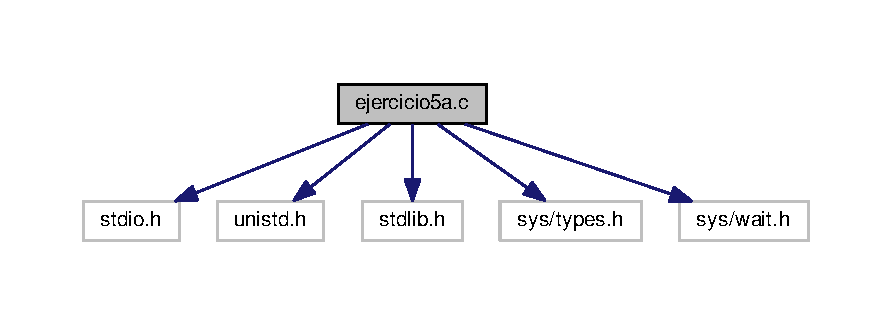
\includegraphics[width=350pt]{ejercicio5a_8c__incl}
\end{center}
\end{figure}
\subsection*{'defines'}
\begin{DoxyCompactItemize}
\item 
\hypertarget{ejercicio5a_8c_acee2369f62e4a096d243dec3cd7d0b00}{\#define {\bfseries N\+U\+M\+\_\+\+P\+R\+O\+C}~3}\label{ejercicio5a_8c_acee2369f62e4a096d243dec3cd7d0b00}

\end{DoxyCompactItemize}
\subsection*{Funciones}
\begin{DoxyCompactItemize}
\item 
\hypertarget{ejercicio5a_8c_a840291bc02cba5474a4cb46a9b9566fe}{int {\bfseries main} (void)}\label{ejercicio5a_8c_a840291bc02cba5474a4cb46a9b9566fe}

\end{DoxyCompactItemize}


\subsection{Descripción detallada}
Fuente del ejercicio 5a. 

Este programa ejecuta una serie de forks de tal forma que un padre solo puede tener un único hijo.

\begin{DoxyAuthor}{Autor}
Pareja 21\+: Juan Riera Gomez (\href{mailto:juan.riera@estudiante.uam.es}{\tt juan.\+riera@estudiante.\+uam.\+es}) y Carlos Ignacio Isasa Martín (\href{mailto:carlos.isasa@estudiante.uam.es}{\tt carlos.\+isasa@estudiante.\+uam.\+es}) 
\end{DoxyAuthor}
\begin{DoxyVersion}{Versión}
1.\+0 
\end{DoxyVersion}
\begin{DoxyDate}{Fecha}
02-\/03-\/2017 
\end{DoxyDate}

\hypertarget{ejercicio5b_8c}{\section{Referencia del Archivo ejercicio5b.\+c}
\label{ejercicio5b_8c}\index{ejercicio5b.\+c@{ejercicio5b.\+c}}
}


Fuente del ejercicio 5b.  


{\ttfamily \#include $<$stdio.\+h$>$}\\*
{\ttfamily \#include $<$stdlib.\+h$>$}\\*
{\ttfamily \#include $<$unistd.\+h$>$}\\*
{\ttfamily \#include $<$sys/types.\+h$>$}\\*
{\ttfamily \#include $<$sys/wait.\+h$>$}\\*
Dependencia gráfica adjunta para ejercicio5b.\+c\+:
\nopagebreak
\begin{figure}[H]
\begin{center}
\leavevmode
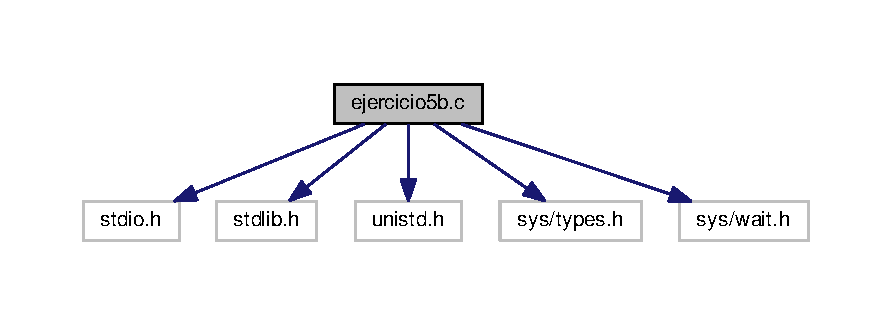
\includegraphics[width=350pt]{ejercicio5b_8c__incl}
\end{center}
\end{figure}
\subsection*{'defines'}
\begin{DoxyCompactItemize}
\item 
\hypertarget{ejercicio5b_8c_acee2369f62e4a096d243dec3cd7d0b00}{\#define {\bfseries N\+U\+M\+\_\+\+P\+R\+O\+C}~3}\label{ejercicio5b_8c_acee2369f62e4a096d243dec3cd7d0b00}

\end{DoxyCompactItemize}
\subsection*{Funciones}
\begin{DoxyCompactItemize}
\item 
\hypertarget{ejercicio5b_8c_a840291bc02cba5474a4cb46a9b9566fe}{int {\bfseries main} (void)}\label{ejercicio5b_8c_a840291bc02cba5474a4cb46a9b9566fe}

\end{DoxyCompactItemize}


\subsection{Descripción detallada}
Fuente del ejercicio 5b. 

Este programa ejecuta una serie de forks de tal forma que un único padre tiene una serie de hijos, pero éstos no tienen más hijos.

\begin{DoxyAuthor}{Autor}
Pareja 21\+: Juan Riera Gomez (\href{mailto:juan.riera@estudiante.uam.es}{\tt juan.\+riera@estudiante.\+uam.\+es}) y Carlos Ignacio Isasa Martín (\href{mailto:carlos.isasa@estudiante.uam.es}{\tt carlos.\+isasa@estudiante.\+uam.\+es}) 
\end{DoxyAuthor}
\begin{DoxyVersion}{Versión}
1.\+0 
\end{DoxyVersion}
\begin{DoxyDate}{Fecha}
02-\/03-\/2017 
\end{DoxyDate}

\hypertarget{ejercicio6_8c}{}\section{Referencia del Archivo ejercicio6.\+c}
\label{ejercicio6_8c}\index{ejercicio6.\+c@{ejercicio6.\+c}}


Fuente del ejercicio 6.  


{\ttfamily \#include $<$stdio.\+h$>$}\\*
{\ttfamily \#include $<$stdlib.\+h$>$}\\*
{\ttfamily \#include $<$sys/ipc.\+h$>$}\\*
{\ttfamily \#include $<$sys/shm.\+h$>$}\\*
{\ttfamily \#include $<$sys/types.\+h$>$}\\*
{\ttfamily \#include $<$unistd.\+h$>$}\\*
{\ttfamily \#include $<$signal.\+h$>$}\\*
{\ttfamily \#include $<$sys/wait.\+h$>$}\\*
{\ttfamily \#include $<$errno.\+h$>$}\\*
{\ttfamily \#include $<$time.\+h$>$}\\*
{\ttfamily \#include $<$string.\+h$>$}\\*
{\ttfamily \#include \char`\"{}semaforos.\+h\char`\"{}}\\*
Dependencia gráfica adjunta para ejercicio6.\+c\+:
\nopagebreak
\begin{figure}[H]
\begin{center}
\leavevmode
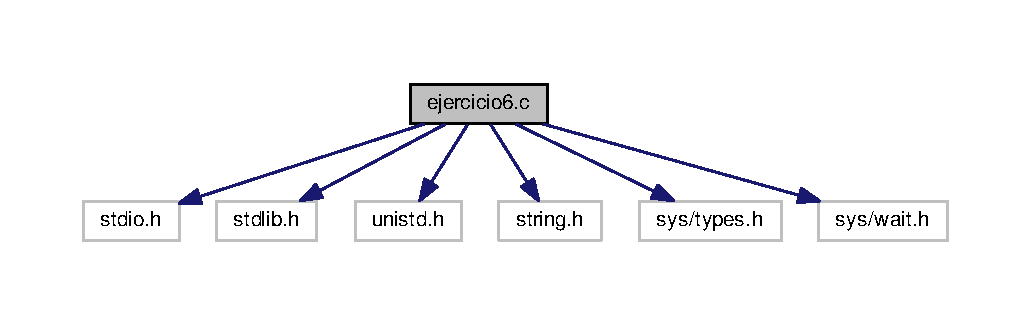
\includegraphics[width=350pt]{ejercicio6_8c__incl}
\end{center}
\end{figure}
\subsection*{\textquotesingle{}defines\textquotesingle{}}
\begin{DoxyCompactItemize}
\item 
\#define {\bfseries M\+A\+X\+B\+UF}~26\hypertarget{ejercicio6_8c_ad7871643c05865c80f5d8050aead2b57}{}\label{ejercicio6_8c_ad7871643c05865c80f5d8050aead2b57}

\item 
\#define {\bfseries P\+R\+O\+J\+ID}~1300\hypertarget{ejercicio6_8c_a489440928d1b279bb8bdc0bb2ccd414f}{}\label{ejercicio6_8c_a489440928d1b279bb8bdc0bb2ccd414f}

\end{DoxyCompactItemize}
\subsection*{Funciones}
\begin{DoxyCompactItemize}
\item 
int {\bfseries main} (int argc, char $\ast$argv\mbox{[}$\,$\mbox{]})\hypertarget{ejercicio6_8c_a0ddf1224851353fc92bfbff6f499fa97}{}\label{ejercicio6_8c_a0ddf1224851353fc92bfbff6f499fa97}

\end{DoxyCompactItemize}


\subsection{Descripción detallada}
Fuente del ejercicio 6. 

En este programa se simula el problema clásico del productor-\/consumidor, un proceso \char`\"{}produce\char`\"{} (escribe en una memoria compartida) y otro \char`\"{}consume\char`\"{} lo que se ha prducido (lee de la memoria compartida lo que ha escrito el productor)

\begin{DoxyAuthor}{Autor}
Juan Riera Gomez (\href{mailto:juan.riera@estudiante.uam.es}{\tt juan.\+riera@estudiante.\+uam.\+es}) y Carlos Ignacio Isasa Martín (\href{mailto:carlos.isasa@estudiante.uam.es}{\tt carlos.\+isasa@estudiante.\+uam.\+es}) 
\end{DoxyAuthor}
\begin{DoxyVersion}{Versión}
1.\+0 
\end{DoxyVersion}
\begin{DoxyDate}{Fecha}
07-\/abril-\/2017 
\end{DoxyDate}

\hypertarget{ejercicio8_8c}{}\section{Referencia del Archivo ejercicio8.\+c}
\label{ejercicio8_8c}\index{ejercicio8.\+c@{ejercicio8.\+c}}


Fuente del ejercicio 8 Este programa pide al usuario un número de procesos y un número de vueltas, estos procesos se pasarán una señal tantas vueltas como pida el usuario. Cada vez que uno la recibe, imprime la hora. Finalmente se acaban uno a uno.  


{\ttfamily \#include $<$stdio.\+h$>$}\\*
{\ttfamily \#include $<$stdlib.\+h$>$}\\*
{\ttfamily \#include $<$string.\+h$>$}\\*
{\ttfamily \#include $<$signal.\+h$>$}\\*
{\ttfamily \#include $<$unistd.\+h$>$}\\*
{\ttfamily \#include $<$sys/types.\+h$>$}\\*
{\ttfamily \#include $<$sys/wait.\+h$>$}\\*
{\ttfamily \#include $<$fcntl.\+h$>$}\\*
{\ttfamily \#include $<$time.\+h$>$}\\*
Dependencia gráfica adjunta para ejercicio8.\+c\+:
\nopagebreak
\begin{figure}[H]
\begin{center}
\leavevmode
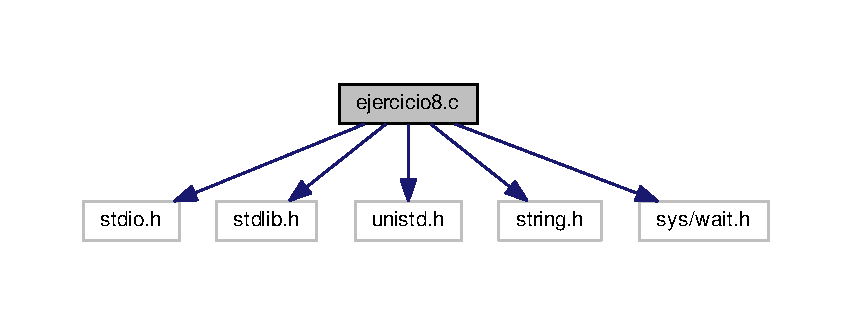
\includegraphics[width=350pt]{ejercicio8_8c__incl}
\end{center}
\end{figure}
\subsection*{Funciones}
\begin{DoxyCompactItemize}
\item 
char $\ast$ {\bfseries tiempo} ()\hypertarget{ejercicio8_8c_a445d4e4144b10aa987da413343200688}{}\label{ejercicio8_8c_a445d4e4144b10aa987da413343200688}

\item 
void {\bfseries manejador\+\_\+sigusr1} (int sig)\hypertarget{ejercicio8_8c_a54e0d453acd2cb0d8adfd611e4158462}{}\label{ejercicio8_8c_a54e0d453acd2cb0d8adfd611e4158462}

\item 
void {\bfseries manejador\+\_\+sigterm} (int sig)\hypertarget{ejercicio8_8c_a7e0d11f7ea2fd257c747e1cea963f357}{}\label{ejercicio8_8c_a7e0d11f7ea2fd257c747e1cea963f357}

\item 
int {\bfseries main} (int argc, char $\ast$argv\mbox{[}$\,$\mbox{]})\hypertarget{ejercicio8_8c_a0ddf1224851353fc92bfbff6f499fa97}{}\label{ejercicio8_8c_a0ddf1224851353fc92bfbff6f499fa97}

\end{DoxyCompactItemize}


\subsection{Descripción detallada}
Fuente del ejercicio 8 Este programa pide al usuario un número de procesos y un número de vueltas, estos procesos se pasarán una señal tantas vueltas como pida el usuario. Cada vez que uno la recibe, imprime la hora. Finalmente se acaban uno a uno. 

\begin{DoxyAuthor}{Autor}
Juan Riera Gomez (\href{mailto:juan.riera@estudiante.uam.es}{\tt juan.\+riera@estudiante.\+uam.\+es}) y Carlos Ignacio Isasa Martín (\href{mailto:carlos.isasa@estudiante.uam.es}{\tt carlos.\+isasa@estudiante.\+uam.\+es}) 
\end{DoxyAuthor}
\begin{DoxyVersion}{Versión}
1.\+0 
\end{DoxyVersion}
\begin{DoxyDate}{Fecha}
15-\/03-\/2017 
\end{DoxyDate}

\hypertarget{ejercicio9_8c}{\section{Referencia del Archivo ejercicio9.\+c}
\label{ejercicio9_8c}\index{ejercicio9.\+c@{ejercicio9.\+c}}
}


Fuente del ejercicio 9.  


{\ttfamily \#include $<$stdio.\+h$>$}\\*
{\ttfamily \#include $<$stdlib.\+h$>$}\\*
{\ttfamily \#include $<$unistd.\+h$>$}\\*
{\ttfamily \#include $<$sys/wait.\+h$>$}\\*
{\ttfamily \#include $<$string.\+h$>$}\\*
Dependencia gráfica adjunta para ejercicio9.\+c\+:
\nopagebreak
\begin{figure}[H]
\begin{center}
\leavevmode
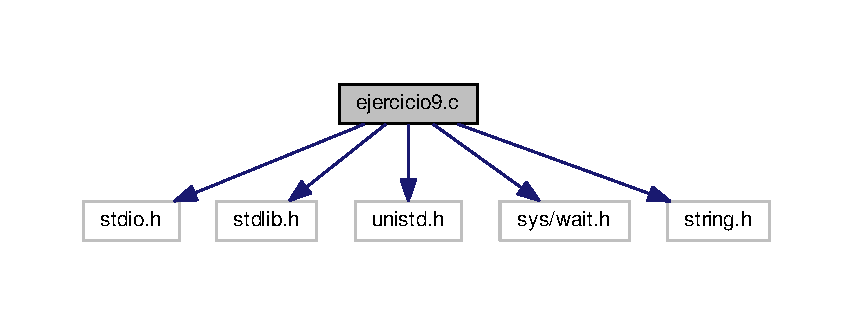
\includegraphics[width=350pt]{ejercicio9_8c__incl}
\end{center}
\end{figure}
\subsection*{'defines'}
\begin{DoxyCompactItemize}
\item 
\hypertarget{ejercicio9_8c_abc8a865f8ec2f1343ebeded8e37b47dc}{\#define {\bfseries L\+E\+E\+R}~0}\label{ejercicio9_8c_abc8a865f8ec2f1343ebeded8e37b47dc}

\item 
\hypertarget{ejercicio9_8c_a1fab98d80466569d31ccf6a35b2c78a6}{\#define {\bfseries E\+S\+C\+R\+I\+B\+I\+R}~1}\label{ejercicio9_8c_a1fab98d80466569d31ccf6a35b2c78a6}

\item 
\hypertarget{ejercicio9_8c_ad7871643c05865c80f5d8050aead2b57}{\#define {\bfseries M\+A\+X\+B\+U\+F}~250}\label{ejercicio9_8c_ad7871643c05865c80f5d8050aead2b57}

\end{DoxyCompactItemize}
\subsection*{Enumeraciones}
\begin{DoxyCompactItemize}
\item 
\hypertarget{ejercicio9_8c_a38327b96c7dded8688dddbc8b14300ad}{enum {\bfseries O\+P\+E\+R\+A\+C\+I\+O\+N} \{ {\bfseries suma} =0, 
{\bfseries resta} =1, 
{\bfseries multi} =2, 
{\bfseries divi} =3
 \}}\label{ejercicio9_8c_a38327b96c7dded8688dddbc8b14300ad}

\end{DoxyCompactItemize}
\subsection*{Funciones}
\begin{DoxyCompactItemize}
\item 
\hypertarget{ejercicio9_8c_ae66f6b31b5ad750f1fe042a706a4e3d4}{int {\bfseries main} ()}\label{ejercicio9_8c_ae66f6b31b5ad750f1fe042a706a4e3d4}

\end{DoxyCompactItemize}


\subsection{Descripción detallada}
Fuente del ejercicio 9. 

Este programa pide al usuario una serie de argumentos por pantalla, después crea cuatro procesos hijo y establece una red de pipes con ellos. Cada uno de estos hijos toma argumentos a través de sus pipes, ejecuta una operación diferente, y devuelve el resultado a través de los pipes. Por último, el proceso padre lee estos resultados y los imprime por pantalla de la forma que haya indicado el usuario por parámetros.

\begin{DoxyAuthor}{Autor}
Pareja 21\+: Juan Riera Gomez (\href{mailto:juan.riera@estudiante.uam.es}{\tt juan.\+riera@estudiante.\+uam.\+es}) y Carlos Ignacio Isasa Martín (\href{mailto:carlos.isasa@estudiante.uam.es}{\tt carlos.\+isasa@estudiante.\+uam.\+es}) 
\end{DoxyAuthor}
\begin{DoxyVersion}{Versión}
1.\+0 
\end{DoxyVersion}
\begin{DoxyDate}{Fecha}
02-\/03-\/2017 
\end{DoxyDate}

%--- End generated contents ---

% Index
\newpage
\phantomsection
\addcontentsline{toc}{chapter}{Índice}
\printindex

\end{document}
